\chapter{Finite element method for the Navier--Stokes equations}\label{ch:fem}
\section{Governing equations}

For reference, we will present here the Navier--Stokes equations, for incompressible Newtonian fluid \cite{Larson-Bengzon}

\begin{align}
  % Conservation of momentum
  \label{eq:NavierStokesConservation}
  \frac{\partial \mathbf{u}(\mathbf{x}, t)}{\partial t} + \left(\mathbf{u}(\mathbf{x}, t)\cdot\nabla\right)\mathbf{u}(\mathbf{x}, t) + \nabla p(\mathbf{x}, t) - \nu\Delta\mathbf{u}(\mathbf{x}, t) &= \mathbf{f}(\mathbf{x}, t)\\
  % Continuity
  \label{eq:NavierStokesContinuity}
  \nabla \cdot \mathbf{u}(\mathbf{x}, t) &= 0
\end{align}
where:
\begin{itemize}
  \item $\mathbf{u} \in \mathbb{R}^n$ is velocity
  \item $p \in \mathbb{R}$ is mechanical pressure
  \item $\nu$ is viscosity
  \item $\mathbf{f}$ represents the body forces acting on the fluid e.g. gravity
\end{itemize}

For the sake of brevity, explicit function parameters will be omitted and body forces will not be considered.

\section{Model problem}
We shall base our studies on the two dimensional DFG benchmark model problem initially presented in \cite{dfg-problem}. It considers flow in a channel with an obstacle. The channel is rectangular with length $2.2$ and height $0.41$. The obstacle is a circle with center at $(0.2, 0.2)$ and diameter $0.1$. \cref{fig:2D_DFG_Benchmark} shows the geometric setup for the benchmark. No-slip boundary condition is imposed on $\Gamma_1 \cup \Gamma_3 \cup \Gamma_5$. Do nothing condition is imposed on $\Gamma_2$. The problem is considered in the time interval $J = \left[0, T\right]$. The viscosity is $\nu = 0.001$. On $\Gamma_4$ we impose Dirichlet boundary condition which determines the type of the flow. Two types of flow will be studied, laminar and turbulent. For laminar flow $\mathbf{u} = \left(\frac{1.2y\left(0.41 - y\right)}{0.41^2}, 0\right), \quad \left(\mathbf{x}, t\right) \in \Gamma_4 \times J$ is imposed. For turbulent flow $\mathbf{u} = \left(\frac{6y(0.41-y)}{0.41^2}, 0\right), \quad \left(\mathbf{x}, t\right) \in \Gamma_4 \times J$ is imposed (see \cref{fig:2D_DFG_Benchmark_BC}).

\begin{figure}[H]
  \centering
  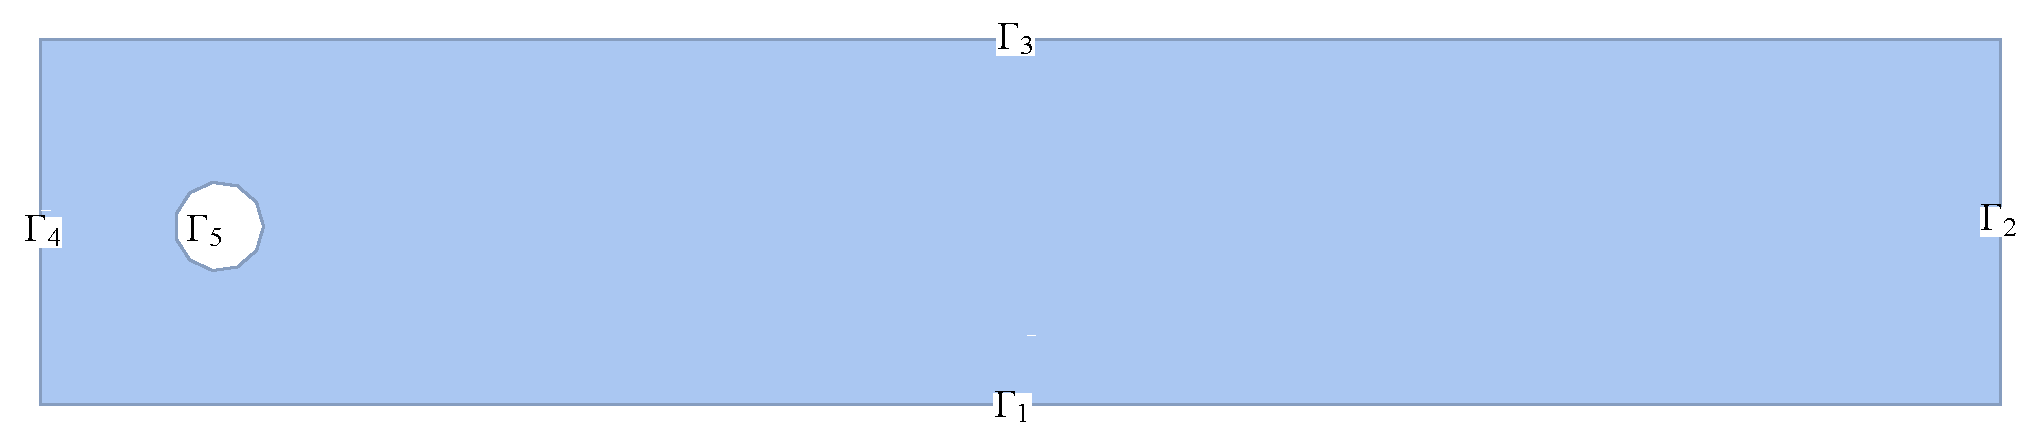
\includegraphics[scale=0.39]{Figures/02_model_problem/2D_DFG_Benchmark.pdf}
  \caption{2D DFG Benchmark setup}
  \label{fig:2D_DFG_Benchmark}
\end{figure}

\begin{figure}[H]
  \centering
  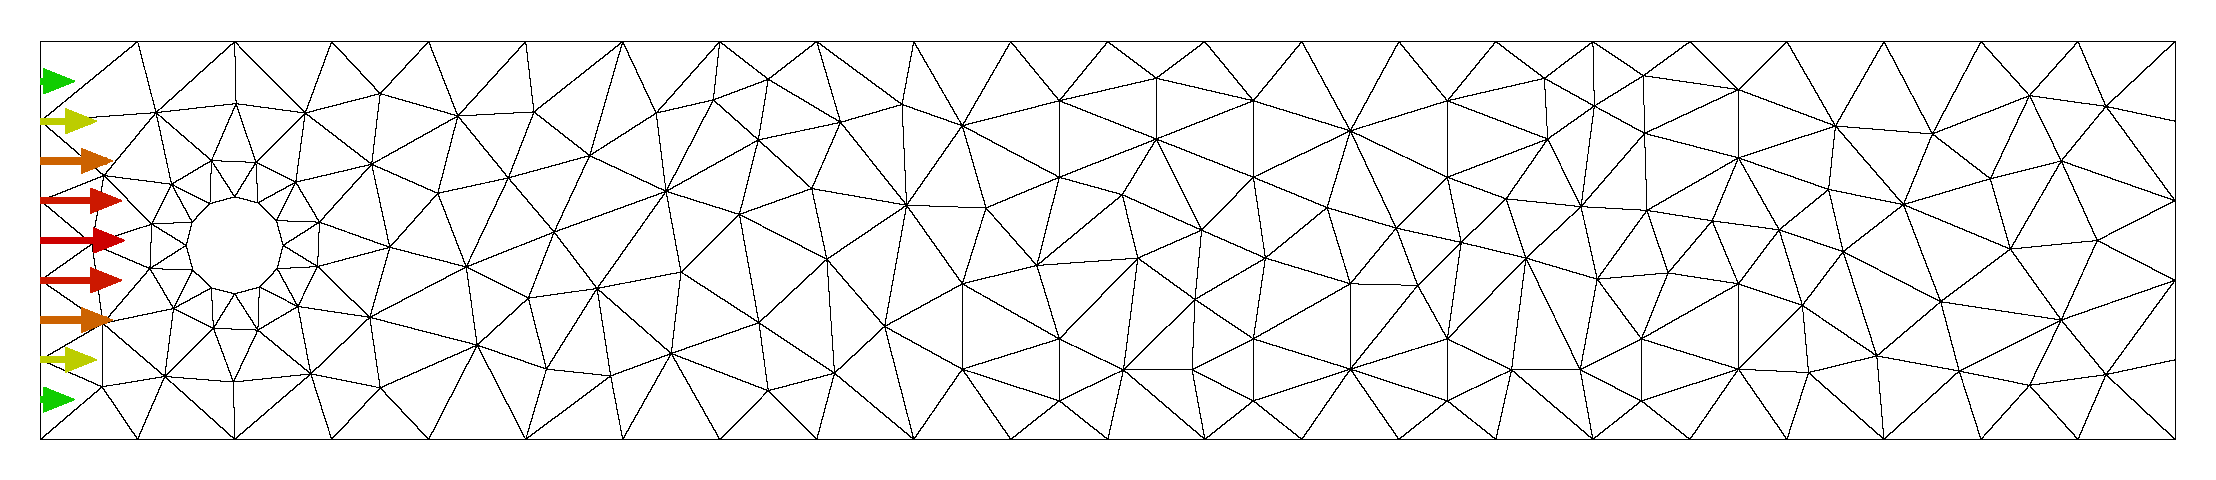
\includegraphics[scale=0.36]{Figures/02_model_problem/dirichlet_conditions.pdf}
  \caption{Dirichlet condition imposed on $\Gamma_4$. It has the same parabolic profile for laminar and turbulent flow. The only difference is in the length of the velocity vector.}
  \label{fig:2D_DFG_Benchmark_BC}
\end{figure}


The differential formulation is now presented. For laminar flow it is:

\begin{equation}
\begin{aligned}
  &\frac{\partial\mathbf{u}}{\partial t} + \mathbf{u} \cdot \nabla\mathbf{u} = -\nabla p + \nu\Delta\mathbf{u}, &&\left(\mathbf{x}, t\right) \in \Omega \times J \\
  &\nabla \cdot \mathbf{u} = 0, &&\left(\mathbf{x}, t\right) \in \Omega \times J \\
  &\mathbf{u} = 0, &&\left(\mathbf{x}, t\right) \in \left(\Gamma_1 \cup \Gamma_3 \cup \Gamma_5\right) \times J \\
  &\mathbf{u} = \left(\frac{1.2y\left(0.41 - y\right)}{0.41^2}, 0\right), &&\left(\mathbf{x}, t\right) \in \Gamma_4 \times J \\
  &\nu\frac{\partial\mathbf{u}}{\partial\mathbf{n}} -p\mathbf{n} = 0, &&\left(\mathbf{x}, t\right) \in \Gamma_2 \times J \\
\end{aligned}\label{eq:laminar_differential_form}
\end{equation}
For turbulent flow it is:
\begin{equation}
\begin{aligned}
  &\frac{\partial\mathbf{u}}{\partial t} + \mathbf{u} \cdot \nabla\mathbf{u} = -\nabla p + \nu\Delta\mathbf{u}, &&\left(\mathbf{x}, t\right) \in \Omega \times J \\
  &\nabla \cdot \mathbf{u} = 0, &&\left(\mathbf{x}, t\right) \in \Omega \times J \\
  &\mathbf{u} = 0, &&\left(\mathbf{x}, t\right) \in \left(\Gamma_1 \cup \Gamma_3 \cup \Gamma_5\right) \times J \\
  &\mathbf{u} = \left(\frac{6y(0.41-y)}{0.41^2}, 0\right), &&\left(\mathbf{x}, t\right) \in \Gamma_4 \times J \\
  &\nu\frac{\partial\mathbf{u}}{\partial\mathbf{n}} -p\mathbf{n} = 0, &&\left(\mathbf{x}, t\right) \in \Gamma_2 \times J \\
\end{aligned}\label{eq:turbulent_differential_form}
\end{equation}

\section{Finite Element Method}
Now, we shall present three FEM-based discretizations of the Navier-Stokes equations. We shall compare them in terms of our main goals -- to find a method that is efficient and easy to parallelize.
\subsection{Direct approach}
One possible way to attack the problem is to consider \cref{eq:laminar_differential_form} or \cref{eq:turbulent_differential_form}, derive a weak formulation and then apply the FEM directly to this weak formulation. Based on \cite{gresho-fem} implicit time integration scheme must be used. A big disadvantage is that this approach requires solving a nonlinear system of equations. The method also requires assembling the convection matrix at each iteration of the nonlinear solver, however, this is not a trivial task to parallelize. The derivation of the FEM will be presented, as well as, the result of a numerical experiment, mainly to outline what the limitations of this approach are for our purposes.
\subsubsection{Weak formulation}
We start by taking the dot products of both sides of the first equation from \cref{eq:laminar_differential_form} with a test function $\mathbf{v} \in V : \left\{\mathbf{v} \in H^1 : \mathbf{v}(\mathbf{x}, t)|_{\Gamma_D} = 0 \right\}$ and both sides of the second equation from \cref{eq:laminar_differential_form} with a test function $p \in L^2(\Omega)$, where $\Gamma_D = \Gamma_1\cup\Gamma_3\cup\Gamma_4\cup\Gamma_5$
\begin{align} \label{eq:2D_DFG_Benchmark_momentum_weak_full}
  &\left(\frac{\partial\mathbf{u}}{\partial t}, \mathbf{v}\right) + (\mathbf{u}\cdot\nabla\mathbf{u}, \mathbf{v}) = -(\nabla p, \mathbf{v}) + \nu(\Delta\mathbf{u}, \mathbf{v}), &&\mathbf{v} \in V \\
  &(\nabla\cdot\mathbf{u}, q) = 0, &&q \in L^2 \\
  &\mathbf{u} = \mathbf{u_{\Gamma_4}}, &&\left(\mathbf{x}, t\right) \in \Gamma_4 \times J
\end{align}
Now for \cref{eq:2D_DFG_Benchmark_momentum_weak_full} we perform integration by parts and obtain:

\begin{align*}
  &\left(\frac{\partial\mathbf{u}}{\partial t}, \mathbf{v}\right)
  + (\mathbf{u}\cdot\nabla\mathbf{u}, \mathbf{v}) = \\
  &(p, \nabla \cdot \mathbf{v})
  - \cancelto{\mathbf{v}|_{\Gamma_D} = 0}{(p\mathbf{n}, \mathbf{v})_{\Gamma_D}}
  - \cancelto{\left(\nu\frac{\partial\mathbf{u}}{\partial\mathbf{n}} - p\mathbf{n}\right)|_{\Gamma_2} = 0}{(p\mathbf{n}, \mathbf{v})_{\Gamma_2}}\\
  &- \nu(\nabla\mathbf{u} : \nabla\mathbf{v})
  + \cancelto{\mathbf{v}|_{\Gamma_D} = 0}{\nu(\mathbf{n}\cdot\nabla\mathbf{u}, \mathbf{v})_{\Gamma_D}}
  + \cancelto{\left(\nu\frac{\partial\mathbf{u}}{\partial\mathbf{n}} - p\mathbf{n}\right)|_{\Gamma_2} = 0}{\nu(\mathbf{n}\cdot\nabla\mathbf{u}, \mathbf{v})_{\Gamma_2}}, \quad \forall\mathbf{v} \in V
\end{align*}
This leads us to the final form of the weak formulation. Find $\mathbf{u}$ and $p$ such that:
\begin{align*}
&\mathbf{u} \in U : \left\{\mathbf{v} \in H^1 : \mathbf{v}(\mathbf{x}, t)|_{\Gamma_1 \cup \Gamma_3 \cup \Gamma_5} = 0\right\} \\
&p \in L^2(\Omega)
\end{align*}
\begin{align}
  \label{eq:2D_DFG_momentum_weak}
  &\left(\frac{\partial\mathbf{u}}{\partial t}, \mathbf{v}\right)
  + (\mathbf{u}\cdot\nabla\mathbf{u}, \mathbf{v}) + \nu(\nabla\mathbf{u} : \nabla\mathbf{v}) =
  (p, \nabla \cdot \mathbf{v}), &&\mathbf{v} \in V \\
  \label{eq:2D_DFG_mass_weak}
  &(\nabla\cdot\mathbf{u}, q) = 0, &&q \in L^2 \\
  &\mathbf{u} = \mathbf{u_{\Gamma_4}}, &&\left(\mathbf{x}, t\right) \in \Gamma_4 \times J  
\end{align}
where the Frobenius inner product of two second rank tensors is a real number, defined as:

\begin{equation*}
	\mathbf{A} : \mathbf{B} = \sum\limits_{i=1}^{n}\sum\limits_{j=1}^{m}A_{i,j}B_{i,j} = A_{i,j}B_{i,j}
\end{equation*}

\subsubsection{Finite Element Method}\label{sec:NS_Direct_Approach_FEM}
Let:
\begin{equation*}
  \{\mathbf{\Phi}_i\}^{2N_v}_{i=1} = \left\{
  \begin{bmatrix} \phi_1 \\ 0\end{bmatrix}
  , \dots ,
  \begin{bmatrix} \phi_{N_v} \\ 0\end{bmatrix}
  ,
  \begin{bmatrix} 0 \\ \phi_1\end{bmatrix}
  , \dots ,
  \begin{bmatrix} 0 \\ \phi_{N_v}\end{bmatrix}
  \right\}
\end{equation*}
be the set of basis functions for the finite dimensional space $U_h$ where we will seek the approximate solution $\mathbf{u}_h$ for the velocity function $\mathbf{u}$ where $N_v$ is the number of velocity nodes in the mesh, which do not lie on $\Gamma_1\cup\Gamma_3\cup\Gamma_5$ and let:

\begin{equation*}
  \left\{\chi_i\right\}^{N_p}_{i = 1}
\end{equation*}
be the set of basis functions for the finite dimensional space $Q_h$ where we will seek the approximate solution $p_h$ for the pressure function $p$ where $N_p$ is the number of pressure nodes in the mesh. Then we can rewrite \cref{eq:2D_DFG_momentum_weak} in terms of the approximate solution. We look for $\mathbf{u}_h$ in the form $\mathbf{u}_h = \sum\limits_{i=1}^{2N_v}{\mathbf{\Phi}_iq_i}$ and $p_h$ in the form $p_h = \sum\limits_{i=1}^{N_p}{\chi_ip_i}$ and, thus, obtain:
{
\newcommand{\SUMU}{\sum\limits_{j=1}^{2N_v}}
\newcommand{\SUMP}{\sum\limits_{j=1}^{N_p}}
\newcommand{\UH}{\SUMU\mathbf{\Phi}_jq_j}
\newcommand{\PH}{\SUMP\mathbf{\chi}_jp_j}
\newcommand{\PHI}[1]{\mathbf{\Phi}_#1}
\newcommand{\ALLI}{\quad \forall i \in [1, 2N_v]}
\begin{multline*}
  \SUMU\frac{dq_j}{dt} \left(\PHI{j}, \PHI{i}\right)
  + \SUMU q_j\left(\mathbf{u}_h\cdot\nabla\PHI{j}, \PHI{i}\right) = \\
  \SUMP p_j\left(\chi_j, \nabla \cdot \PHI{i}\right)
  - \nu\SUMU q_j\left(\nabla\PHI{j} : \nabla\PHI{i}\right), \ALLI
\end{multline*}
}
More precisely, the latter equations should hold for all $i$, corresponding to nodes, which don't lie on $\Gamma_D$. The system is closed by imposing the Dirichlet boundary conditions on $\Gamma_4$. However, we shall neglect this for the time being, and explain later how we impose the Dirichlet boundary conditions in practice. From \cref{eq:2D_DFG_mass_weak} we have:
{
\newcommand{\ALLI}{\quad \forall i \in [1, N_p]}
\newcommand{\SUMU}{\sum\limits_{j=1}^{2N_v}}
\newcommand{\UH}{\SUMU\mathbf{\Phi}_jq_j}
\begin{align*}
  \SUMU q_j\left(\nabla\cdot\mathbf{\Phi}_j, \chi_i\right) = 0, \ALLI
\end{align*}
}
Now putting these in matrix form, we finally obtain:
\begin{multline}\label{eq:FEM-Matrix-Form}
  \begin{bmatrix}
  \mathbf{M} & 0 & 0 \\
  0 & \mathbf{M} & 0 \\
  0 & 0 & 0
  \end{bmatrix}
  \begin{bmatrix}
  \dot{\mathbf{q}}_1\\
  \dot{\mathbf{q}}_2\\
  \mathbf{p}
  \end{bmatrix}
  =
  \begin{bmatrix}
  -\nu\mathbf{K} - \mathbf{C(u_h)} & 0 & \mathbf{B}^T_1 \\
  0 & -\nu\mathbf{K} - \mathbf{C(u_h)} & \mathbf{B}^T_2 \\
  \mathbf{B}_1 & \mathbf{B}_2 & 0
  \end{bmatrix}
  \begin{bmatrix}
  \mathbf{q}_1\\
  \mathbf{q}_2\\
  \mathbf{p}
  \end{bmatrix}
\end{multline}
where $\mathbf{M}$ denotes the mass matrix, which can be lumped.
\begin{equation*}
	\mathbf{M} =
	\begin{bmatrix}
		\left(\phi_1, \phi_1\right) & \left(\phi_2, \phi_1\right) & \cdots & \left(\phi_{N_v}, \phi_1\right) \\
		\left(\phi_1, \phi_2\right) & \left(\phi_2, \phi_2\right) & \cdots & \left(\phi_{N_v}, \phi_2\right) \\
		\vdots & \vdots & \cdots & \vdots \\
		\left(\phi_1, \phi_{N_v}\right) & \left(\phi_2, \phi_{N_v}\right) & \cdots & \left(\phi_{N_v}, \phi_{N_v}\right)
	\end{bmatrix}
\end{equation*}
$\mathbf{C}$ denotes the convection matrix, which depends on the fluid velocities:
\begin{equation*}
	\mathbf{C}(\mathbf{u}_h) = \begin{bmatrix}
		\left(\mathbf{u}_h\cdot\nabla\phi_1, \phi_1\right) & \left(\mathbf{u}_h\cdot\nabla\phi_2, \phi_1\right) & \cdots & \left(\mathbf{u}_h\cdot\nabla\phi_{N_v}, \phi_1\right)\\
		\left(\mathbf{u}_h\cdot\nabla\phi_1, \phi_2\right) & \left(\mathbf{u}_h\cdot\nabla\phi_2, \phi_2\right) & \cdots & \left(\mathbf{u}_h\cdot\nabla\phi_{N_v}, \phi_2\right)\\
		\vdots & \vdots & \cdots & \vdots \\
		\left(\mathbf{u}_h\cdot\nabla\phi_1, \phi_{N_v}\right) & \left(\mathbf{u}_h\cdot\nabla\phi_2, \phi_{N_v}\right) & \cdots & \left(\mathbf{u}_h\cdot\nabla\phi_{N_v}, \phi_{N_v}\right)
	\end{bmatrix}
\end{equation*}
$\mathbf{K}$ denotes the stiffness matrix:
\begin{equation*}
	\mathbf{K} = \begin{bmatrix}
		\left(\nabla\phi_1\cdot\nabla\phi_1\right) & \left(\nabla\phi_2\cdot\nabla\phi_1\right) &
		\cdots &
		\left(\nabla\phi_{N_v}\cdot\nabla\phi_1\right) \\
		\left(\nabla\phi_1\cdot\nabla\phi_2\right) & \left(\nabla\phi_2\cdot\nabla\phi_2\right) &
		\cdots &
		\left(\nabla\phi_{N_v}\cdot\nabla\phi_2\right) \\
		\vdots & \vdots & \cdots & \vdots \\
		\left(\nabla\phi_1\cdot\nabla\phi_{N_v}\right) & \left(\nabla\phi_2\cdot\nabla\phi_{N_v}\right) &
		\cdots &
		\left(\nabla\phi_{N_v}\cdot\nabla\phi_{N_v}\right)
	\end{bmatrix}
\end{equation*}

\begin{equation*}
	\mathbf{B}_1 = \begin{bmatrix}
		\left(\frac{\partial\phi_1}{\partial x_1}, \chi_1\right) & \left(\frac{\partial\phi_2}{\partial x_1}, \chi_1\right) & \cdots & \left(\frac{\partial\phi_{N_v}}{\partial x_1}, \chi_1\right) \\
		\left(\frac{\partial\phi_1}{\partial x_1}, \chi_2\right) & \left(\frac{\partial\phi_2}{\partial x_1}, \chi_2\right) & \cdots & \left(\frac{\partial\phi_{N_v}}{\partial x_1}, \chi_2\right) \\
		\vdots & \vdots & \cdots & \vdots \\
		\left(\frac{\partial\phi_1}{\partial x_1}, \chi_{N_p}\right) & \left(\frac{\partial\phi_2}{\partial x_1}, \chi_{N_p}\right) & \cdots & \left(\frac{\partial\phi_{N_v}}{\partial x_1}, \chi_{N_p}\right)
	\end{bmatrix}
\end{equation*}

\begin{equation*}
\mathbf{B}_2 = \begin{bmatrix}
\left(\frac{\partial\phi_1}{\partial x_2}, \chi_1\right) & \left(\frac{\partial\phi_2}{\partial x_2}, \chi_1\right) & \cdots & \left(\frac{\partial\phi_{N_v}}{\partial x_2}, \chi_1\right) \\
\left(\frac{\partial\phi_1}{\partial x_2}, \chi_2\right) & \left(\frac{\partial\phi_2}{\partial x_2}, \chi_2\right) & \cdots & \left(\frac{\partial\phi_{N_v}}{\partial x_2}, \chi_2\right) \\
\vdots & \vdots & \cdots & \vdots \\
\left(\frac{\partial\phi_1}{\partial x_2}, \chi_{N_p}\right) & \left(\frac{\partial\phi_2}{\partial x_2}, \chi_{N_p}\right) & \cdots & \left(\frac{\partial\phi_{N_v}}{\partial x_2}, \chi_{N_p}\right)
\end{bmatrix}
\end{equation*}

\subsubsection{Time discretization}
For the time discretization Crank-Nicolson method is used:

\begin{gather*}
	\begin{bmatrix}
		\mathbf{M} & 0 & 0 \\
		0 & \mathbf{M} & 0 \\
		0 & 0 & 0
	\end{bmatrix}
	\left(\begin{bmatrix}
		\mathbf{Q}_1^{i+1}\\
		\mathbf{Q}_2^{i+1}\\
		\mathbf{P}^{i+1}
	\end{bmatrix}
	-
	\begin{bmatrix}
		\mathbf{Q}_1^{i}\\
		\mathbf{Q}_2^{i}\\
		\mathbf{P}^{i}
	\end{bmatrix}\right)
	\frac{1}{\Delta t}
	= \\
	\frac{1}{2}
	\begin{bmatrix}
	-\nu\mathbf{K} - \mathbf{C}(\mathbf{u}_h^{i+1}) & 0 & \mathbf{B}^T_1 \\
	0 & -\nu\mathbf{K} - \mathbf{C}(\mathbf{u}_h^{i+1}) & \mathbf{B}^T_2 \\
	\mathbf{B}_1 & \mathbf{B}_2 & 0
	\end{bmatrix}
	\begin{bmatrix}
	\mathbf{Q}_1^{i+1}\\
	\mathbf{Q}_2^{i+1}\\
	\mathbf{P}^{i+1}
	\end{bmatrix}\\
	+\frac{1}{2}\begin{bmatrix}
	-\nu\mathbf{K} - \mathbf{C}(\mathbf{u}_h^i) & 0 & \mathbf{B}^T_1 \\
	0 & -\nu\mathbf{K} - \mathbf{C}(\mathbf{u}_h^i) & \mathbf{B}^T_2 \\
	\mathbf{B}_1 & \mathbf{B}_2 & 0
	\end{bmatrix}
	\begin{bmatrix}
	\mathbf{Q}_1^i\\
	\mathbf{Q}_2^i\\
	\mathbf{P}^i
	\end{bmatrix}
\end{gather*}
which leads to the following nonlinear system of equations:
\begin{multline}\label{eq:2D_DFG_Direct_Crank-Nicholson}
	\begin{bmatrix}
		\mathbf{M}+\frac{\Delta t}{2}\left(\nu\mathbf{K}+\mathbf{C}(\mathbf{u}_h^{i+1})\right) & 0 & -\frac{\Delta t}{2}\mathbf{B}^T_1 \\
		0 &\mathbf{M}+\frac{\Delta t}{2}\left(\nu\mathbf{K}+\mathbf{C}(\mathbf{u}_h^{i+1})\right) & -\frac{\Delta t}{2}\mathbf{B}^T_2 \\
		-\frac{\Delta t}{2}\mathbf{B}_1 & -\frac{\Delta t}{2}\mathbf{B}_2 & 0
	\end{bmatrix}
	\begin{bmatrix}
		\mathbf{Q}_1^{i+1}\\
		\mathbf{Q}_2^{i+1}\\
		\mathbf{P}^{i+1}
	\end{bmatrix} = \\
	\begin{bmatrix}
		\mathbf{M}-\frac{\Delta t}{2}\left(\nu\mathbf{K}+\mathbf{C}(\mathbf{u}_h^{i})\right) & 0 & \frac{\Delta t}{2}\mathbf{B}^T_1 \\
		0 &\mathbf{M}-\frac{\Delta t}{2}\left(\nu\mathbf{K}+\mathbf{C}(\mathbf{u}_h^{i})\right) & \frac{\Delta t}{2}\mathbf{B}^T_2 \\
		\frac{\Delta t}{2}\mathbf{B}_1 & \frac{\Delta t}{2}\mathbf{B}_2 & 0
	\end{bmatrix}
	\begin{bmatrix}
		\mathbf{Q}_1^{i}\\
		\mathbf{Q}_2^{i}\\
		\mathbf{P}^{i}
	\end{bmatrix}
\end{multline}
This system is solved via Picard iteration.

\subsubsection{Dirichlet Boundary Conditions}
In order to impose the boundary conditions on $\Gamma_D$ we shall assemble the matrices as if the nodes on $\Gamma_D$ were "regular" nodes, then the matrix and the right hand side of \cref{eq:2D_DFG_Direct_Crank-Nicholson} will be tweaked. Let us denote the matrix on the left-hand-side of \cref{eq:2D_DFG_Direct_Crank-Nicholson} with $A$ and the vector on the right-hand-side of \cref{eq:2D_DFG_Direct_Crank-Nicholson} with $\mathbf{b}$. Then \cref{alg:impose-diriclet} shows how to tweak \cref{eq:2D_DFG_Direct_Crank-Nicholson} in order to apply the Dirichlet boundary conditions and preserve the symmetry of the matrix.

\begin{algorithm}[H]
\centering
\caption{Impose Dirichlet Boundary Conditions}\label{alg:impose-diriclet}
\begin{algorithmic}[1]
		\Procedure{ImposeDirichlet}{$dirichletIndices, values, A, \mathbf{b}$}
			\ForAll{j $\in$ dirichletIndices}
				\State Set the $j-th$ row of $A$ to 0
				\State $A[j][j] \gets 1$
				\State $b[j] \gets values[j]$
				\ForAll{$i \neq j$ row in A}
					\State $b[i] \gets b[i] - values[j]*A[i][j]$
					\State $A[i][j] \gets 0$
				\EndFor
			\EndFor
		\EndProcedure
\end{algorithmic}
\end{algorithm}

\subsection{Operator Splitting}
As it was mentioned in the introduction according to \cite{gresho-fem} only implicit time discretization methods for \cref{eq:FEM-Matrix-Form} make sense. On the other hand, using implicit time discretization methods for \cref{eq:FEM-Matrix-Form} would require solving nonlinear systems at each time step which is an extremely computationally expensive process. Furthermore, it would not be trivial to parallelize the method, presented in the previous chapter, for our purposes. Thus another technique, which is commonly applied and allows for the use of explicit time approximation will be presented. The trick is to split the differential operator (with respect to time). The method proposed in \cite{Chorin-operator-split} splits the operator in two, while the one proposed in \cite{Bridson} splits it in three. Both splitting techniques will require solving an equation in which the second derivative of the pressure will be present. This means that the element's polynomial space for the pressure must be at least of first order.

\subsubsection{Chorin Split}
The first approach which will be presented will split the differential operator in time into two parts. One part which governs the velocity and another which governs the pressure. We start by approximating \cref{eq:NavierStokesConservation} with forward difference and then adding and subtracting a dummy term in the forward difference.

\begin{align*}
	\frac{\vecf{u}^{i+1} - \vecf{u}^{i}}{\Delta t} + \vecf{u}^i \cdot \nabla\vecf{u}^i + \nabla p^i - \nu \Delta \vecf{u}^i &= 0 \\
		\frac{\vecf{u}^{i+1} + \vecf{u}^{i+\frac{1}{2}} - \vecf{u}^{i+\frac{1}{2}} - \vecf{u}^{i}}{\Delta t} + \vecf{u}^i \cdot \nabla\vecf{u}^i + \nabla p^i - \nu \Delta \vecf{u}^i &= 0
\end{align*}
Now we can split the equations. At one fraction of time the pressure will be computed and at the other everything else.

\begin{align}
	\frac{\vecf{u}^{i + \frac{1}{2}} - \vecf{u}^{i}}{\Delta t} &= \nu \Delta \vecf{u}^i - \vecf{u}^i \cdot \nabla\vecf{u}^i \label{eq:chorin_tentative_velocity}\\
	\frac{\vecf{u}^{i+1} - \vecf{u}^{i + \frac{1}{2}}}{\Delta t} &= - \nabla p^i \label{eq:chorin_pressure_before_split}
\end{align}
Now we can further transform \cref{eq:chorin_pressure_before_split}, by taking the divergence of both sides. From \cref{eq:NavierStokesContinuity} we know that $\divg{\vecf{u}^{i+1}} = 0$. And we get:

\begin{equation*}
	\divg{\vecf{u}^{i + \frac{1}{2}}} = \lapl{p^i} \Delta t
\end{equation*}
known as the Pressure Poisson Equation.

The most controversial part of this splitting are the boundary conditions. For the velocity we shall impose the corresponding no-slip boundary conditions on $\Gamma_1 \cup \Gamma_3 \cup \Gamma_5$, on the outflow boundary $\Gamma_2$ we shall impose $\vecf{n} \cdot \grad{\vecf{u}^i} = 0$ and on the inflow boundary $\Gamma_4$ a constant velocity $\mathbf{u}_{\Gamma_4}$ is imposed. For the pressure we shall impose $\vecf{n} \cdot \grad{p^i} = 0$ on $\Gamma_1 \cup \Gamma_3 \cup \Gamma_4 \cup \Gamma_5$. Imposing $\vecf{n} \cdot \grad{p^i} = 0$ has no physical meaning and is believed to lead to bad approximation of the pressure near the boundary \cite{Larson-Bengzon}. For the pressure on the outflow boundary we shall impose $p^i = 0$. This is done in order to mimic the do-nothing boundary condition.

Finally, the equations to which we shall apply the FEM are:
\begin{align}
	&\frac{\vecf{u}^{i + \frac{1}{2}} - \vecf{u}^{i}}{\Delta t} = \nu \Delta \vecf{u}^i - \vecf{u}^i \cdot \nabla\vecf{u}^i, && \left(\mathbf{x}, t\right) \in \Omega \times J \label{eq:NS_PPE_Final_Split_advect} \\
	&\divg{\vecf{u}^{i + \frac{1}{2}}} = \lapl{p^i} \Delta t, && \left(\mathbf{x}, t\right) \in \Omega \times J  \label{eq:NS_PPE_Final_Split_PPE} \\
	&\vecf{u}^{i+1} = \vecf{u}^{i+\frac{1}{2}} - \Delta t \grad{p^{i}}, && \left(\mathbf{x}, t\right) \in \Omega \times J\label{eq:NS_Final_Split_final_velocity}  \\
  &\vecf{n} \cdot \grad{\vecf{u}^i} = 0, && \left(\mathbf{x}, t\right) \in \Gamma_2 \times J \\
  &\vecf{u}^i = 0, &&\left(\mathbf{x}, t\right) \in \left(\Gamma_1 \cup \Gamma_3 \cup \Gamma_5\right) \times J \\
  &\vecf{u}^i = \vecf{u}_{\Gamma_4}, && \left(\mathbf{x}, t\right) \in \Gamma_4 \times J \\
  &\vecf{n} \cdot \grad{p^i} = 0, && \left(\mathbf{x}, t\right) \in (\Gamma_1 \cup \Gamma_3 \cup \Gamma_4 \cup \Gamma_5) \times J \\
  &p^i = 0, && \left(\mathbf{x}, t\right) \in \Gamma_2 \times J
\end{align}

\paragraph{Weak formulation}
We begin with \cref{eq:NS_PPE_Final_Split_advect}. As usual both sides of the equation are multiplied by a test function $\mathbf{v} \in V = \{\vecf{v} \vert \vecf{v} \in H^1 \land \vecf{v}|_{\Gamma_D} = 0\}$

\begin{align*}
	\dotprod{\frac{\vecf{u}^{i + \frac{1}{2}} - \vecf{u}^{i}}{\Delta t}}{\vecf{v}} &= \dotprod{\nu\lapl{\vecf{u}^i}}{\vecf{v}} - \dotprod{\vecf{u}^i \cdot \grad{\vecf{u}^i}}{\vecf{v}}, \forall\mathbf{v} \in V \\
	\dotprod{\frac{\vecf{u}^{i + \frac{1}{2}} - \vecf{u}^{i}}{\Delta t}}{\vecf{v}} &= \cancelto{\vecf{v}|_{\Gamma_D} = \vecf{0}}{\nu\dotprod{\vecf{n} \cdot \grad{\vecf{u}}}{\vecf{v}}_{\Gamma_D}} + \cancelto{\left(\vecf{n} \cdot \grad{\vecf{u}^i}\right)|_{\Gamma_2} = 0}{\nu\dotprod{\vecf{n} \cdot \grad{\vecf{u}}}{\vecf{v}}_{\Gamma_2}}  \\&- \nu\left(\grad{\vecf{u}^i} : \grad{\vecf{v}}\right) - \dotprod{\vecf{u}^i \cdot \grad{\vecf{u}^i}}{\vecf{v}}, \forall\mathbf{v} \in V \\
	\dotprod{\vecf{u}^{i + \frac{1}{2}}}{\vecf{v}} &= \dotprod{\vecf{u}^i}{\vecf{v}} - \Delta t \left[\nu\left(\grad{\vecf{u}^i} : \grad{\vecf{v}}\right) + \dotprod{\vecf{u}^i \cdot \grad{\vecf{u}^i}}{\vecf{v}}\right], \forall\mathbf{v} \in V \\
\end{align*}

Next we shall multiply both sides of \cref{eq:NS_PPE_Final_Split_PPE} with a test function $q \in Q = \{q\vert q \in H^1 \land q|_{\Gamma_2} = 0\}$.

\begin{align*}
	\dotprod{\divg{\vecf{u}^{i + \frac{1}{2}}}}{q} &= \Delta t\dotprod{\lapl{p^i}}{q}, \forall q \in Q \\
	\dotprod{\divg{\vecf{u}^{i + \frac{1}{2}}}}{q} & = \cancelto{\left(\vecf{n} \cdot \grad{p^i}\right)|_{\Gamma_D} = 0}{\Delta t\dotprod{\vecf{n} \cdot \grad{p^i}}{q}\vert_{\Gamma_D}} + \cancelto{q|_{\Gamma_D} = 0}{\Delta t\dotprod{\vecf{n} \cdot \grad{p^i}}{q}\vert_{\Gamma_D}} - \Delta t \dotprod{\grad{p^i}}{\grad{q}}, \forall q \in Q \\
	\dotprod{\divg{\vecf{u}^{i + \frac{1}{2}}}}{q} &= - \Delta t \dotprod{\grad{p^i}}{\grad{q}}, \forall q \in Q
\end{align*}

Finally we take the dot product of both sides of \cref{eq:NS_Final_Split_final_velocity} with a test function $\vecf{v} \in V$.
$$
\dotprod{\vecf{u}^{i+1}}{\vecf{v}} = \dotprod{\vecf{u}^{i+\frac{1}{2}}}{\vecf{v}} - \Delta t\dotprod{\vecf{v}} {\grad{p^i}}
$$
\paragraph{Finite Element Method}
We shall seek the approximate solution $\mathbf{u}_h$ and $p_h$ in a finite dimensional subspaces of $V$ and $Q$. Let us use the same notation for the basis functions of those spaces as in \cref{sec:NS_Direct_Approach_FEM}.
\begin{equation}
\begin{aligned}
	\begin{bmatrix}
		\mathbf{M} & 0 \\
		0 & \mathbf{M}
	\end{bmatrix}
	\begin{bmatrix}
		\vecf{Q^{i + \frac{1}{2}}_1} \\
		\vecf{Q^{i + \frac{1}{2}}_2}
	\end{bmatrix} &=
	\begin{bmatrix}
		\mathbf{M} & 0 \\
		0 & \mathbf{M}
	\end{bmatrix}
	\begin{bmatrix}
		\vecf{Q^{i}_1} \\
		\vecf{Q^{i}_2}
	\end{bmatrix} - \Delta t \begin{bmatrix}
		\nu \mathbf{K} + \mathbf{C}(\vecf{u_h}) & 0 \\
		0 & \nu \mathbf{K} + \mathbf{C}(\vecf{u_h})
	\end{bmatrix} \begin{bmatrix}
		\vecf{Q^i_1} \\
		\vecf{Q^i_2}
	\end{bmatrix} \\
	\mathbf{K_p}\vecf{P}^i &= -\frac{1}{\Delta t} \begin{bmatrix}
		\mathbf{B_1} & \mathbf{B_2}
	\end{bmatrix} \begin{bmatrix}
		\vecf{Q^{i + \frac{1}{2}}_1} \\
		\vecf{Q^{i + \frac{1}{2}}_2}
	\end{bmatrix} \\
	\begin{bmatrix}
		\mathbf{M} & 0 \\
		0 & \mathbf{M}
	\end{bmatrix} \begin{bmatrix}
		\vecf{Q^{i+1}_1} \\
		\vecf{Q^{i+1}_2}
	\end{bmatrix} &=	\begin{bmatrix}
		\mathbf{M} & 0 \\
		0 & \mathbf{M}
	\end{bmatrix} \begin{bmatrix}
		\vecf{Q^{i+\frac{1}{2}}_1} \\
		\vecf{Q^{i+\frac{1}{2}}_2}
	\end{bmatrix} - \Delta t \begin{bmatrix}
		\vecf{B_{p,1}} \\
		\vecf{B_{p,2}}
	\end{bmatrix} \vecf{P}^i
\end{aligned}\label{eq:chorin_split_fem}
\end{equation}
where $\mathbf{K_p}$ is given by:

\begin{equation*}
	\mathbf{K_p} = \begin{bmatrix}
		\dotprod{\grad{\chi_1}}{\grad{\chi_1}} & \dotprod{\grad{\chi_2}}{\grad{\chi_1}} & \dots & \dotprod{\grad{\chi_{Np}}}{\grad{\chi_1}}\\
		\dotprod{\grad{\chi_1}}{\grad{\chi_2}} & \dotprod{\grad{\chi_2}}{\grad{\chi_2}} & \dots & \dotprod{\grad{\chi_{Np}}}{\grad{\chi_2}}\\
		\vdots & \vdots & \vdots & \vdots\\
		\dotprod{\grad{\chi_1}}{\grad{\chi_{Np}}} & \dotprod{\grad{\chi_2}}{\grad{\chi_{Np}}} & \dots & \dotprod{\grad{\chi_{Np}}}{\grad{\chi_{Np}}}
	\end{bmatrix}
\end{equation*}
$\mathbf{B_{p,1}}$ is given by:

\begin{equation*}
	\mathbf{B_{p,1}} = \begin{bmatrix}
		\left(\frac{\partial\chi_1}{\partial x_1}, \phi_1\right) & \left(\frac{\partial\chi_2}{\partial x_1}, \phi_1\right) & \cdots & \left(\frac{\partial\chi_{N_p}}{\partial x_1}, \phi_1\right) \\
		\left(\frac{\partial\chi_1}{\partial x_1}, \phi_2\right) & \left(\frac{\partial\chi_2}{\partial x_1}, \phi_2\right) & \cdots & \left(\frac{\partial\chi_{N_p}}{\partial x_1}, \phi_2\right) \\
		\vdots & \vdots & \cdots & \vdots \\
		\left(\frac{\partial\chi_1}{\partial x_1}, \phi_{N_v}\right) & \left(\frac{\partial\chi_2}{\partial x_1}, \phi_{N_v}\right) & \cdots & \left(\frac{\partial\chi_{N_v}}{\partial x_1}, \phi_{N_v}\right)
	\end{bmatrix}
\end{equation*}
$\mathbf{B_{p,2}}$ is given by:

\begin{equation*}
	\mathbf{B_{p,2}} = \begin{bmatrix}
		\left(\frac{\partial\chi_1}{\partial x_2}, \phi_1\right) & \left(\frac{\partial\chi_2}{\partial x_2}, \phi_1\right) & \cdots & \left(\frac{\partial\chi_{N_p}}{\partial x_2}, \phi_1\right) \\
		\left(\frac{\partial\chi_1}{\partial x_2}, \phi_2\right) & \left(\frac{\partial\chi_2}{\partial x_2}, \phi_2\right) & \cdots & \left(\frac{\partial\chi_{N_p}}{\partial x_2}, \phi_2\right) \\
		\vdots & \vdots & \cdots & \vdots \\
		\left(\frac{\partial\chi_1}{\partial x_2}, \phi_{N_v}\right) & \left(\frac{\partial\chi_2}{\partial x_2}, \phi_{N_v}\right) & \cdots & \left(\frac{\partial\chi_{N_v}}{\partial x_2}, \phi_{N_v}\right)
	\end{bmatrix}
\end{equation*}

The Dirichlet boundary conditions are imposed in practice in the usual way.

\subsubsection{Advection--Diffusion split}
The Chorin split is easy to implement but it has some flaws. One of them is the fact that the diffusion is approximated with an explicit scheme. This ties the time step to the space step (element size). In case more spatial detail is needed and the spatial mesh is refined we must lower the time step in order to have a stable method. This property is not desired, at least in computer graphics, because videos are produced with a specific frame per second ratio, so the frames produced when the time step is lowered will not be used, this is a waste of time and computational resources. One thing we could do is to approximate the diffusion--advection part of the equation with an implicit scheme. This would require solving a nonlinear system on each time step, which is also not desired. One can try to work around this problem by trying a semi-implicit scheme. Instead of doing that we shall do another split of the differential operator with respect to time, and split the diffusion and advection into separate equations. This split has two advantages -- first, as we show later, there exists an efficient, embarrassingly parallel algorithm which can be used for the advection equation. Second, the diffusion can be approximated with an implicit scheme, without the need to solve nonlinear system at each time step. We shall derive the equation the same way that the Chorin split was derived. This time however we shall add and subtract two dummy variables $\vecf{u^A}$ and $\vecf{u^B}$.

\begin{align}
	&\frac{\vecf{u}^{i+1} - \vecf{u}^{i}}{\Delta t} + \vecf{u}^i \cdot \nabla\vecf{u}^i + \nabla p^i - \nu \Delta \vecf{u}^i &= 0 \\
	&\frac{\vecf{u}^{i+1} + \vecf{u^A} - \vecf{u^A} + \vecf{u^B} - \vecf{u^B} - \vecf{u}^{i}}{\Delta t} + \vecf{u}^i \cdot \nabla\vecf{u}^i + \nabla p^i - \nu \Delta \vecf{u}^i &= 0\label{eq:advection-diffusion-before-split}
\end{align}
Now we shall split \cref{eq:advection-diffusion-before-split} into three separate parts, keeping in mind that we want to use the implicit Euler method for the diffusion equation.
\begin{align*}
	&\frac{\vecf{u^A} - \vecf{u}^i}{\Delta t} + \vecf{u}^i \cdot \nabla\vecf{u}^i = 0 \\
	&\frac{\vecf{u^B} - \vecf{u^A}}{\Delta t} =\nu \Delta \vecf{u^B}\\
	&\frac{\vecf{u}^{i+1} - \vecf{u^B}}{\Delta t} = -\nabla p^i
\end{align*}
The pressure term is treated the same way, by taking the divergence of both sides, as in the Chorin split. The system of equations which should be solved is:
\begin{align}
	&\frac{\vecf{u^A} - \vecf{u}^i}{\Delta t} + \vecf{u}^i \cdot \nabla\vecf{u}^i = 0, &&\left(\mathbf{x}, t\right) \in \Omega \times J \label{eq:general-three-way-split-advection} \\
	&\frac{\vecf{u^B} - \vecf{u^A}}{\Delta t} = \nu \Delta \vecf{u^B}, &&\left(\mathbf{x}, t\right) \in \Omega \times J\\
	&\divg{\vecf{u^B}} = \lapl{p^i} \Delta t, &&\left(\mathbf{x}, t\right) \in \Omega \times J\\
	&\vecf{u}^{i+1} = \vecf{u^B} - \Delta t \grad{p^{i}}, &&\left(\mathbf{x}, t\right) \in \Omega \times J \\
	&\vecf{n} \cdot \grad{\vecf{u}^i} = 0, && \left(\mathbf{x}, t\right) \in \Gamma_2 \times J \\
	&\vecf{u}^i = 0, &&\left(\mathbf{x}, t\right) \in \left(\Gamma_1 \cup \Gamma_3 \cup \Gamma_5\right) \times J \\
	&\vecf{u}^i = \vecf{u}_{\Gamma_4}, && \left(\mathbf{x}, t\right) \in \Gamma_4 \times J \\
	&\vecf{n} \cdot \grad{p^i} = 0, && \left(\mathbf{x}, t\right) \in (\Gamma_1 \cup \Gamma_3 \cup \Gamma_4 \cup \Gamma_5) \times J \\
	&p^i = 0, && \left(\mathbf{x}, t\right) \in \Gamma_2 \times J
\end{align}
Note that this is slightly different than the split applied in \cite{Bridson}. In their approach the advection is first, then the pressure projection is applied, then the diffusion is applied. This requires another pressure projection step after the diffusion in order to impose incompresibillity. This way both the advection and the diffusion are performed in a divergence free fluid. On the other hand, formally, only $\vecf{u}^{i+1}$ is required to be noncompressible and that is why we do not apply the pressure projection step twice. Our numerical experiment does not show problems with the accuracy or the stability of our approach. More experiments are needed, however.
\paragraph{Semi-Lagrangian Advection}
One problem \cref{eq:general-three-way-split-advection} has is the stability of the advection phase. The FEM discretization would not be stable in C norm. There are various ways to improve the stability of the FEM, some of them are presented in \cite{gresho-fem}. However, there is another downside of using the finite element method for solving \cref{eq:general-three-way-split-advection} -- at each time step we must assemble the convection matrix. While the time needed for the assembly is not much compared to the time spent in the Conjugate Gradient method, it is a fact that matrix assembly procedures do not scale well when processor count is increased. Most of the algorithms used for multithreading assembly procedures are based on graph coloring, which is a NP-Complete problem, moreover the coloring would depend on the numbering of elements and nodes.

For solving the advection equation, we shall use the semi-Lagrangian method, a stable method \cite{semi-lagrangian-stability} which falls under the category of embarrassingly parallel of algorithms. Which means that, at least in theory, the algorithm should scale linearly when processor count is increased. It does not require using any locking mechanisms and is suitable to be implemented on a GPU.

Solving \cref{eq:general-three-way-split-advection} in a Lagrangian framework is trivial. Assume we were simulating each particle individually, then \cref{eq:general-three-way-split-advection} would be trivially satisfied when we move all particles, which are being simulated. Finding the velocity for a particular particle is also trivial, because we would have all particles with their velocities explicitly stored in some structure. Working directly with particles has its downsides, however. We must either change our mesh at each point in time or we have to use some tree-like structure to handle the movement and creation of particles. To cope with this problem we shall use a mixture of Eulerian and Lagrangian frameworks (thus the name semi-Lagrangian). Let us demonstrate the idea with an example.

\begin{figure}[H]
	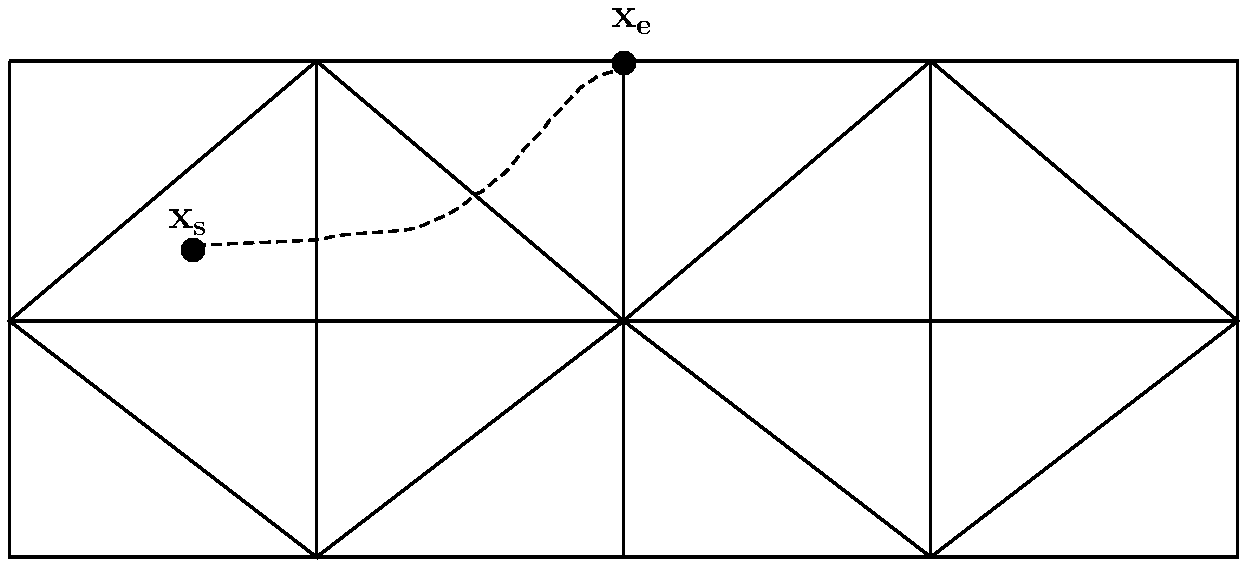
\includegraphics[width=\linewidth]{Figures/semi-lagrangian.pdf}
	\caption{Semi-Lagrangian Method}
	\label{fig:semi-lagrangian}
\end{figure}

Looking at \cref{fig:semi-lagrangian} we want to find the velocity (or any other quantity which is being advected) at time $t + \Delta t$ at point $\mathbf{x_e}$. In a Lagrangian framework this would be the same as the velocity of the (same) particle which at time $t$ was at $\mathbf{x_s}$ and has moved to $\mathbf{x_e}$ at time $t + \Delta t$. So our first problem is how to find $\mathbf{x_s}$. In order to do so we will linearize the velocity field go ``backwards'' in it. Let us elaborate, in a Lagrangian framework \cref{eq:general-three-way-split-advection} boils down to:

\begin{equation*}
	\frac{\partial\mathbf{x}}{\partial t} = \mathbf{u}
\end{equation*}
which we choose to approximate with a backward difference.

\begin{align*}
	\frac{\mathbf{x_e} - \mathbf{x_s}}{\Delta t} &= \mathbf{u}(\mathbf{x_e}, t) \\
	\mathbf{x_s} &= \mathbf{x_e} - \Delta t \mathbf{u}(\mathbf{x_e}, t)
\end{align*}

Now that we have found out the starting position of our imaginary particle, we are presented with another problem. We are not working in a Lagrangian framework and we are not simulating particles and it is almost certain that $\mathbf{x_s}$ will not be a vertex in our Eluerian mesh. The obvious solution is to interpolate the value inside the element using the values we have. Moreover it can be proven \cite{semi-lagrangian-stability} that the method is stable when we interpolate the value inside the element which surrounds it, the same cannot be stated if we decide to extrapolate and use values from elements which do not contain $\mathbf{x_s}$. In case $\mathbf{x_s}$ lies outside of the mesh we find the closest point on the boundary and take its value instead. Note that the position we found by this procedure is not the exact position of the particle which would end up in $\mathbf{x_e}$ beacuse we have used the velocity at $(\mathbf{x_e}, t)$ to approximate the velocity at $(\mathbf{x_e}, t + \Delta t)$, (see \cite{semi-lagrangian-stability} for an error estimate of this approach.)

The type of the mesh is of great importance when implementing the semi-Lagrangian algorithm. There are two properties of the mesh which we should consider. First is the shape of the element and the second is whether the mesh is structured. The term structured mesh is somewhat loose, by this we mean mesh whose elements have the same orientation and the same size, so that the indices of adjacent elements and nodes can be expressed via some explicit formula. An example of structured mesh with rectangular elements would be \cref{fig:structured-mesh}

\begin{figure}[H]
	\centering
	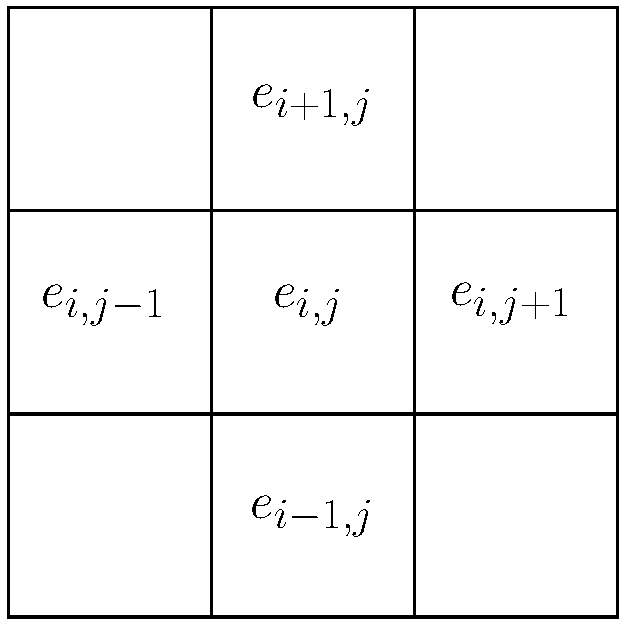
\includegraphics[width=0.4\linewidth]{Figures/structured-mesh.pdf}
	\caption{Structured mesh with rectangular elements.}\label{fig:structured-mesh}
\end{figure}

The advantage in working with such meshes (especially ones with rectangular elements) is that it is easy to find in which element a point lies. It all boils down to simple integer arithmetics. However when the mesh is unstructured we must iterate through all elements in order to find where a point lies. In our case we are working with unstructured triangular mesh. For this reason KD Tree data structure was implemented in order to accelerate the process of finding which element of the mesh contain a given point. It has complexity of $O(\log{n})$ for searching (assuming the tree is balanced) which element contains a point where $n$ is the total number of elements. Also it has another useful property: it can accelerate finding of the closest mesh point to another arbitrary point, although the worst case has complexity $O(n)$ it is rarely reached and on average it has complexity $O(\log{n})$. Assuming a KD Tree is implemented and filled with the elements of the mesh, a pseudo code for the advection phase is presented.

\begin{algorithm}[H]
\centering
\caption{Semi-Lagrangian Advection}\label{alg:Semi-Lagrangian-Advection}
\begin{algorithmic}[1]
		\Procedure{advect}{$KDTree, nodesIn, \Delta t$}
			\State $nodesOut \gets nodesIn$
			\ForAll{velocityNode $\in$ nodesIn}
				\State $\vecf{x_s} \gets velocityNode.position - velocityNode.velocity\Delta t $
				\If{$pointInMesh(KDTree, \vecf{x_s})$}
					\State $element \gets findElement(KDTree, \vecf{x_s})$
					\State $nodesOut.velocity \gets interpolate(\vecf{x_s}, element.velocityNodes)$
				\Else
					\State $closestVelocityNode \gets findClosestNode(KDTree, \vecf{x_s})$
					\State $nodesOut.velocity \gets closestVelocityNode.velocity$
				\EndIf
			\EndFor
		\EndProcedure
		\Return nodesOut
\end{algorithmic}
\end{algorithm}

\paragraph{Finite Element Method}
Now that we have a stable algorithm for the advection phase we can state the Finite Element Method for the given three way split using implicit Euler method for the diffusion.


\begin{align}
	&\mathbf{Q^A} = advect(KDTree, \mathbf{Q^{i}}, \Delta t) \label{eq:_adv-diff-split-advect}\\
		&\left(\begin{bmatrix}
		\mathbf{M} & 0 \\
		0 & \mathbf{M}
	\end{bmatrix} + \nu\Delta t\begin{bmatrix}
		\mathbf{K} & 0 \\
		0 & \mathbf{K}
	\end{bmatrix}\right)\begin{bmatrix}
		\vecf{Q^{B}_1} \\
		\vecf{Q^{B}_2}
	\end{bmatrix} = \begin{bmatrix}
		\mathbf{M} & 0 \\
		0 & \mathbf{M}
	\end{bmatrix}\begin{bmatrix}
		\vecf{Q^{A}_1} \\
		\vecf{Q^{A}_2}
	\end{bmatrix} \label{eq:_adv-diff-split-diffuse}\\
	&\mathbf{K_p}\vecf{P}^i = -\frac{1}{\Delta t} \begin{bmatrix}
		\mathbf{B_1} & \mathbf{B_2}
	\end{bmatrix} \begin{bmatrix}
		\vecf{Q^{B}_1} \\
		\vecf{Q^{B}_2}
	\end{bmatrix} \label{eq:_adv-diff-split-pressure}\\
	&\begin{bmatrix}
		\mathbf{M} & 0 \\
		0 & \mathbf{M}
	\end{bmatrix} \begin{bmatrix}
		\vecf{Q^{i+1}_1} \\
		\vecf{Q^{i+1}_2}
	\end{bmatrix} =	\begin{bmatrix}
		\mathbf{M} & 0 \\
		0 & \mathbf{M}
	\end{bmatrix} \begin{bmatrix}
		\vecf{Q^{B}_1} \\
		\vecf{Q^{B}_2}
	\end{bmatrix} - \Delta t \begin{bmatrix}
		\vecf{B_{p,1}} \\
		\vecf{B_{p,2}}
	\end{bmatrix} \vecf{P}^i \label{eq:_adv-diff-split-velicity-mass}
\end{align}
where \cref{eq:_adv-diff-split-advect} uses \cref{alg:Semi-Lagrangian-Advection}.

Again, the Dirichlet BC are imposed in the usual way.

\subsection{Choice of elements}

Now we shall present the elements used in this work. First of all, let us note that generating a FEM mesh is a large subject on its own and falls out of the scope of this work. Wolfram Mathematica was used to generate the FEM meshes used here. As of this date there is no built-in way to generate curved isoparametric elements with Wolfram Mathematica. For the direct approach we have used the $P_{-1}P_0$ non-conforming Crouzeix-Raviart element (see \cref{fig:P1P0-CR-Standard}). While it does not satisfy the LBB condition it can be proven \cite{Larson-Bengzon} that it is stable. It has the advantage of being divergence free and is computationally cheap. Using $P_{-1}P_0$ with the direct approach will produce a smaller matrix, compared to using any higher order element, thus the non-linear solver should perform better. For the two operator splitting methods $P_2P_1$ (see \cref{fig:P2P1-Standard}) Taylor-Hood element was used, it satisfies the LBB condition and according to \cite{gresho-fem} it is ``the simplest second order element'' and an ``early favorite''.

\begin{figure}[H]
  \centering
  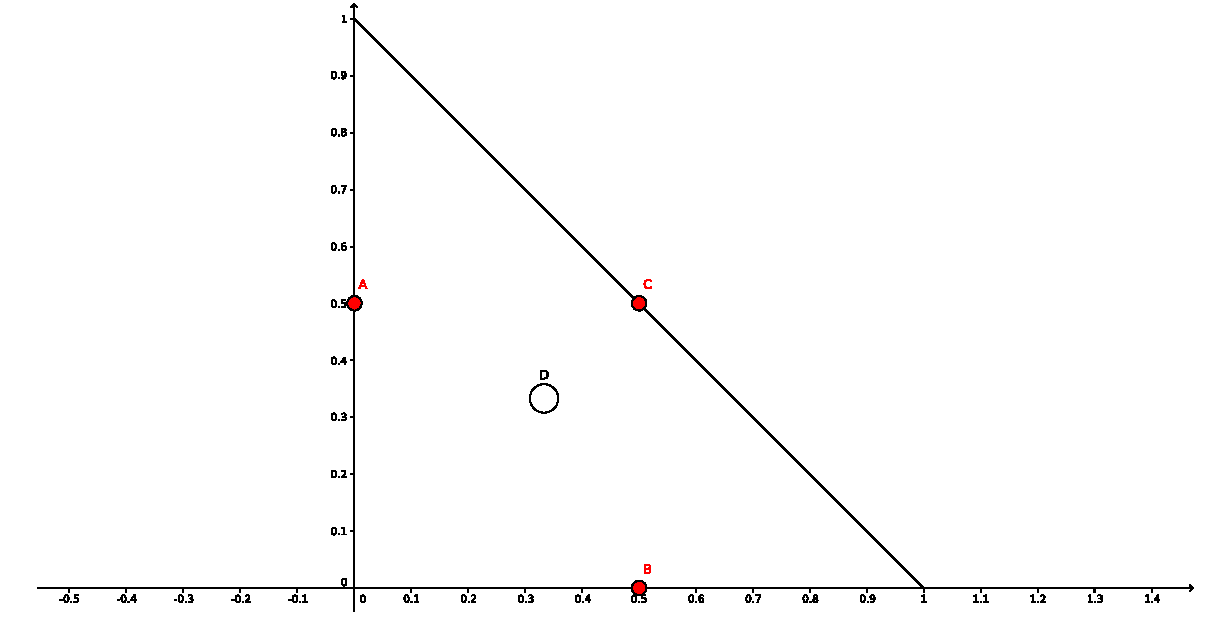
\includegraphics[width=\textwidth]{Figures/01_introduction/cr_element.pdf}
  \caption{$P_{-1}P_0$ non-conforming Crouzeix-Raviart standard element. The 3 degrees of freedom for the velocity are marked with a solid color, the single degree of freedom for the pressure is marked with a circle.}\label{fig:P1P0-CR-Standard}
\end{figure}

\begin{figure}[H]
  \centering
  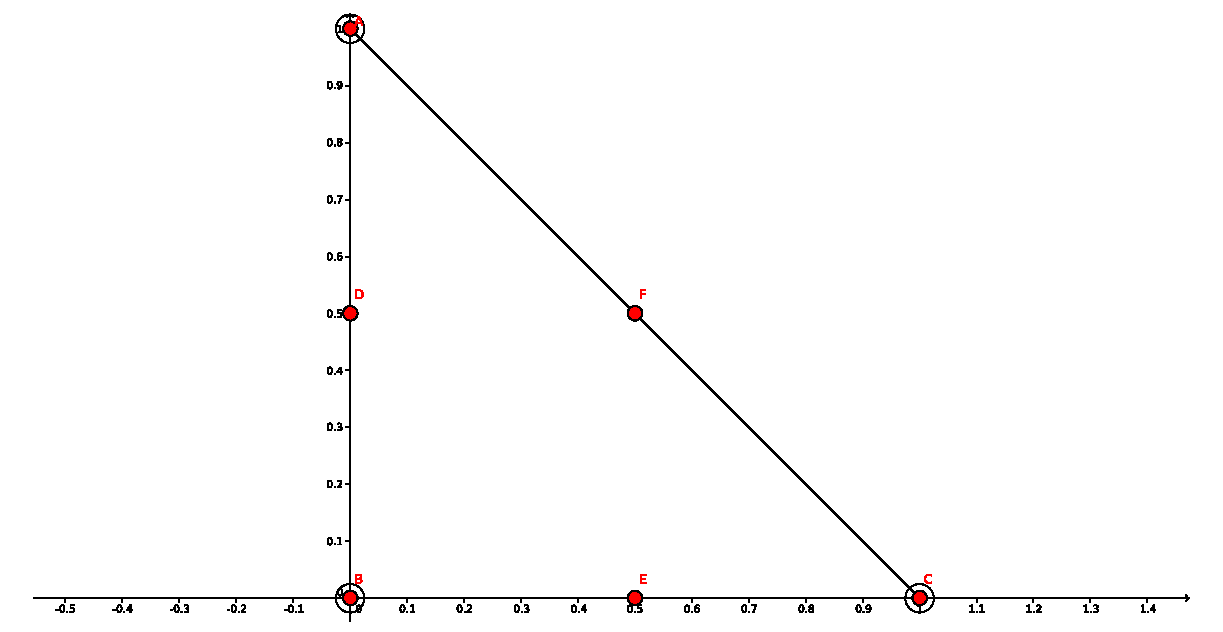
\includegraphics[width=\textwidth]{Figures/01_introduction/tylor_hood_element.pdf}
  \caption{$P_2P_1$ Taylor-Hood standard element. The 6 degrees of freedom for the velocity are marked with a solid color, the 3 degrees of freedom for the pressure are marked with a circle.}\label{fig:P2P1-Standard}
\end{figure}

\section{The CSR sparse matrix format}
We have chosen store the FEM matrices in the Compressed Sparse Row (CSR) format, which we shall describe briefly. For more information about other sparse matrix formats (see \cite{saad-sparse}). Let us denote the number of nonzero elements in a matrix with $nnz$ and the number of rows with $m$. The CSR format consists of 3 arrays, one real array \textit{NZ} of size $nnz$ containing the nonzero entries of the matrix, one integer array \text{Pos} of size $nnz$ containing the column for each nonzero entry and one integer array \text{Start} of size $m + 1$ containing the start index in \text{Pos} for each row of the matrix, the last element of the \text{Start} is usually an integer number equal to $nnz$. We note that the rows are sorted by their index in increasing fashion, but there is no such requirement of the columns and they can be stored in an arbitrary fashion, however for this work we choose to sort the columns in each row in increasing fashion, because this imporoves the cache locality in the computer implementation. Let us illustrate the format with an example, by applying it to the following matrix (see \cref{fig:example_sparse_matrix}).
\begin{figure}[H]
$$
\begin{bmatrix}
	1 & 0 & 0 & 2 & 0\\
	0 & 0 & 3 & 4 & 0\\
	0 & 0 & 5 & 0 & 6\\
	0 & 0 & 0 & 0 & 0\\
	7 & 0 & 8 & 9 & 0
\end{bmatrix}
$$
\caption{Example sparse matrix}\label{fig:example_sparse_matrix}
\end{figure}
The matrix stored in CSR format is shown in \cref{fig:example_csr_sparse_matrix}

\begin{figure}[H]
\centering
\begin{tabular}{l|ccccccccc}
\cline{2-10}
\textit{NZ}    & 1 & 2 & 3 & 4 & 5 & 6                      & 7 & 8 & \multicolumn{1}{c|}{9} \\ \cline{2-10}
\textit{Pos}   & 0 & 3 & 2 & 3 & 2 & 4                      & 0 & 2 & \multicolumn{1}{c|}{3} \\ \cline{2-10}
\textit{Start} & 0 & 2 & 4 & 6 & 6 & \multicolumn{1}{c|}{9} &   &   &                        \\ \cline{2-7}
\end{tabular}\caption{The matrix from \cref{fig:example_sparse_matrix} stored in CSR format. The indexing of the columns and the rows starts from 0.}\label{fig:example_csr_sparse_matrix}
\end{figure}

The memory needed to store a matrix in CSR format is $O(2*nnz + m)$. The space saved by compressing repeating row indexes turns out to be non-negligible \cite{saad-sparse}.

The number of nonzero elements in row $i$ can be found by $Start[i+1] - Start[i]$, the format allows for having empty rows, then $Start[i+1] - Start[i] = 0$. To find the next row with nonzero entries one shall iterate to find the first $i$ for which the $Start[i+1] - Start[i] \neq 0$.

This format is not flexible. Adding and removing nonzero entries after the sparse matrix is initialized would require shifting the \textit{NZ} and \textit{Pos} arrays with $O(nnz)$ time complexity and updating the values in the \textit{Start} array for $O(m)$, yielding total of $O(2*nnz) + O(m)$ operations which is considered to be slow. Despite the lack of flexibility this format allows for efficient implementation of matrix vector multiplication (see \cite{saad-sparse}).

\section{Solving Linear Systems of Equations}
Usually systems of equations which arise when applying numerical methods for differential equations have sparse matrices. This is true for the matrices in \crefrange{eq:_adv-diff-split-diffuse}{eq:_adv-diff-split-velicity-mass} and for the matrix in \cref{eq:2D_DFG_Direct_Crank-Nicholson}. In the course of this work various methods for solving linear systems with sparse matrices were studied. In this section we shall consider solving \crefrange{eq:_adv-diff-split-diffuse}{eq:_adv-diff-split-velicity-mass} which have symmetric positive definite matrices. Systems with such matrices are most commonly solved using the Conjugate Gradient method, which we shall discuss in this section. For information about sparse matrix formats and other methods for solving linear systems (which might be needed should \cref{eq:2D_DFG_Direct_Crank-Nicholson} be considered for solving the differential problem) refer to \cite{saad-sparse}.

\subsection{Conjugate Gradient}
The Conjugate Gradient method is one of the most famous and most studied methods for solving linear systems. It is part of the Krylov family of methods. The method is a special case of Incomplete Orthogonalization Method. In the case of SPD matrices it can be shown that each new direction can be represented with a short recurrency, thus only 3 vectors should be stored at a time. For full derivation and detailed explanation of the method refer to \cite{saad-sparse}. Here we shall present only pseudocode for the method.

\begin{algorithm}[H]
\centering
\caption{Conjugate Gradient Method solving $Ax=b$ with an initial guess $x_0$}\label{alg:CG}
\begin{algorithmic}[1]
		\Procedure{CG}{$A, b, x_0$}
			\State $r_0 \gets b - Ax_0$
			\State $p_0 \gets r_0$
			\For{$j \gets 0, 1, \dots$ until convergence}
				\State $\alpha_j \gets \frac{(r_j, r_j)}{(Ap_j, p_j)}$
				\State $x_{j+1} \gets x_j + \alpha_j p_j$
				\State $r_{j+1} \gets r_j - \alpha_j Ap_j$
				\State $\beta_j \gets \frac{(r_{j+1}, r_{j+1})}{(r_j, r_j)}$
				\State $p_{j+1} \gets r_{j+1} + \beta_j p_j$
			\EndFor
			\State \Return $x_{j+1}$
		\EndProcedure
\end{algorithmic}
\end{algorithm}

\subsection{Zero Fill-in Incomplete Cholesky Preconditioner (IC0)}
The point of preconditioning is to improve the condition number of the matrix. Using a good preconditioner can significantly lower the number of iterations needed by the method to converge. A good preconditioner for the CG method should not change the properties of the matrix and keep it SPD. Let us assume that such a preconditioner is used. Multiplying two sparse matrices often produces a dense matrix, thus it is not wise to precondition the system by directly multiplying the matrix. A better approach incorporates the preconditioner in each iteration. There are few ways to do so in the CG with a preconditioner which is also SPD. The following algorithm is one of those proposed in \cite{saad-sparse}.

\begin{algorithm}[H]
\centering
\caption{Preconditioned Conjugate Gradient Method solving $Ax=b$ with an initial guess $x_0$}\label{alg:pcg}
\begin{algorithmic}[1]
		\Procedure{PCG}{$A, M^{-1} b, x_0$}
			\State $r_0 \gets b - Ax_0$
			\State $z_0 \gets M^{-1}r_0$\label{alg-line:apply-preconditioner}
			\State $p_0 \gets z_0$
			\For{$j \gets 0, 1, \dots$ until convergence}
				\State $\alpha_j \gets \frac{(r_j, z_j)}{(Ap_j, p_j)}$
				\State $x_{j+1} \gets x_j + \alpha_j p_j$
				\State $r_{j+1} \gets r_j - \alpha_j Ap_j$
				\State $z_{j+1} \gets M^{-1}r_{j+1}$
				\State $\beta_j \gets \frac{(r_{j+1}, z_{j+1})}{(r_j, z_j)}$
				\State $p_{j+1} \gets z_{j+1} + \beta_j p_j$
			\EndFor
			\State \Return $x_{j+1}$
		\EndProcedure
\end{algorithmic}
\end{algorithm}

Given \cref{alg:pcg} a logical choice for a preconditioner is the Cholesky decomposition of the matrix $A = LL^T$. However we are not guaranteed that $L$ will be sparse even when $A$ is. Thus we want to find $\widetilde{L}$ which is close to $L$ and $\widetilde{L}\widetilde{L}^T$ which is close to $A$. We choose $\widetilde{L}$ such that it has the same nonzero pattern as the lower triangular part of $A$. This preconditioner can be computed via the standard Cholesky decomposition procedure by dropping elements $l_{i,j}$ for i and j such that $a_{i,j} = 0$. Now when the preconditioner and the matrix share the same non-zero pattern the preconditioner could be represented only by its values. We choose to store $\widetilde{L}^T$ in order to make the memory access more regular and improve the performance.

\section{Numerical Experiment}
Let us now show the plot of the solution of \cref{eq:laminar_differential_form}, afther the 100 iterations with step $\Delta t = 0.01$, produced by solving \cref{eq:2D_DFG_Direct_Crank-Nicholson} and compare it to the solution of the same differential problem, but solved by solving \cref{eq:chorin_split_fem} with $\Delta t = 0.01$ and\crefrange{eq:_adv-diff-split-advect}{eq:_adv-diff-split-velicity-mass} with $\Delta t = 0.01$.\footnote{There is a stylistic difference between \cref{fig:p0p1-plot}, \cref{fig:chorin-plot} and \cref{fig:advection-diffusion-plot}. This is because the solutions for the direct approach and the Chorin split were obtained by a prototype written in Wolfram Mathematica while the last plot was produced by the final version of the code written in C++ and CUDA.} We can observe that \cref{eq:chorin_split_fem}  and \crefrange{eq:_adv-diff-split-advect}{eq:_adv-diff-split-velicity-mass} produce similar results, while solving \cref{eq:2D_DFG_Direct_Crank-Nicholson} with $P_{-1}P_0$ element produces worse results, especially near the boundaries. It must be noted, however, that this comparison is not completely honest, because the two splitting methods use higher order elements. A solution of \cref{eq:laminar_differential_form} with the LBB unstable $P_1P_1$ element could be found in \cite{Larson-Bengzon}. It is also better than the result achieved by \cref{eq:2D_DFG_Direct_Crank-Nicholson}. This leads us to believe that an element of at least first degree polynomial space should be used for the pressure. The compuational cost of solving nonlinear systems and the bad results produced with $P_{-1}P_0$ element have discouraged us from further investigation of \cref{eq:2D_DFG_Direct_Crank-Nicholson}.

\begin{figure}[H]
\centering
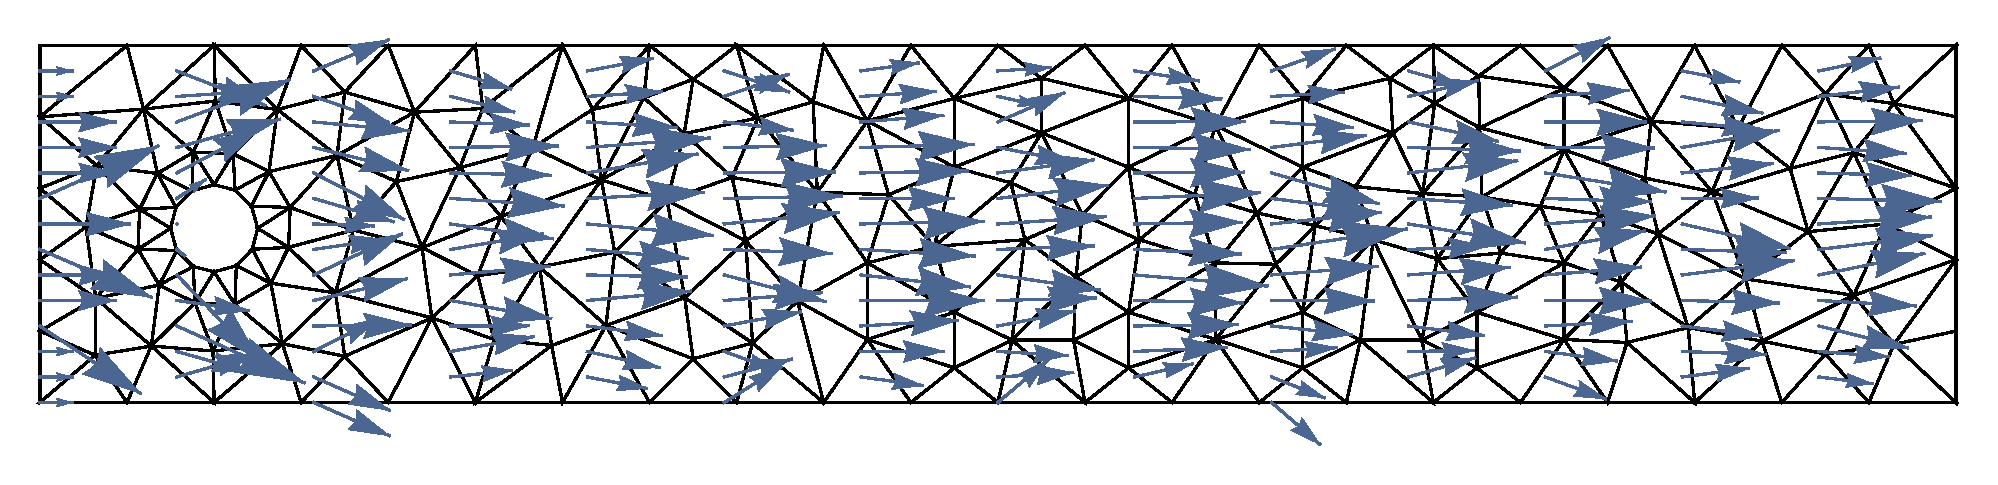
\includegraphics[width=\textwidth]{Figures/01_introduction/P1P0_100.pdf}
\caption{Solution for laminar flow via \cref{eq:2D_DFG_Direct_Crank-Nicholson} after 100 iterations with $\Delta t = 0.01$ }\label{fig:p0p1-plot}
\end{figure}

\begin{figure}[H]
\centering
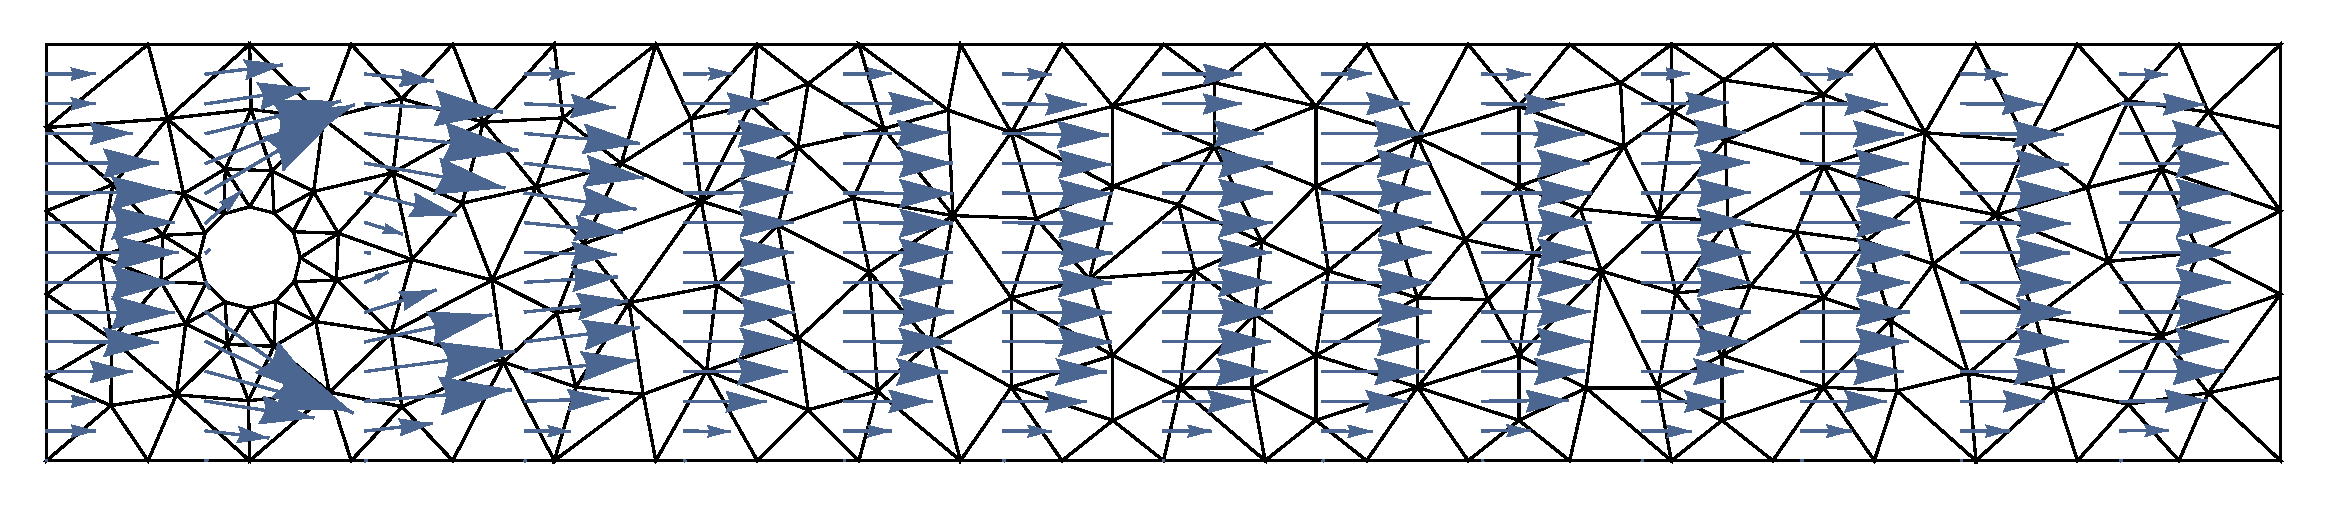
\includegraphics[width=\textwidth]{Figures/01_introduction/P2P1_100.pdf}
\caption{Solution for laminar flow via \cref{eq:chorin_split_fem} after 100 iterations with $\Delta t = 0.01$ }\label{fig:chorin-plot}
\end{figure}

\begin{figure}[H]
\centering
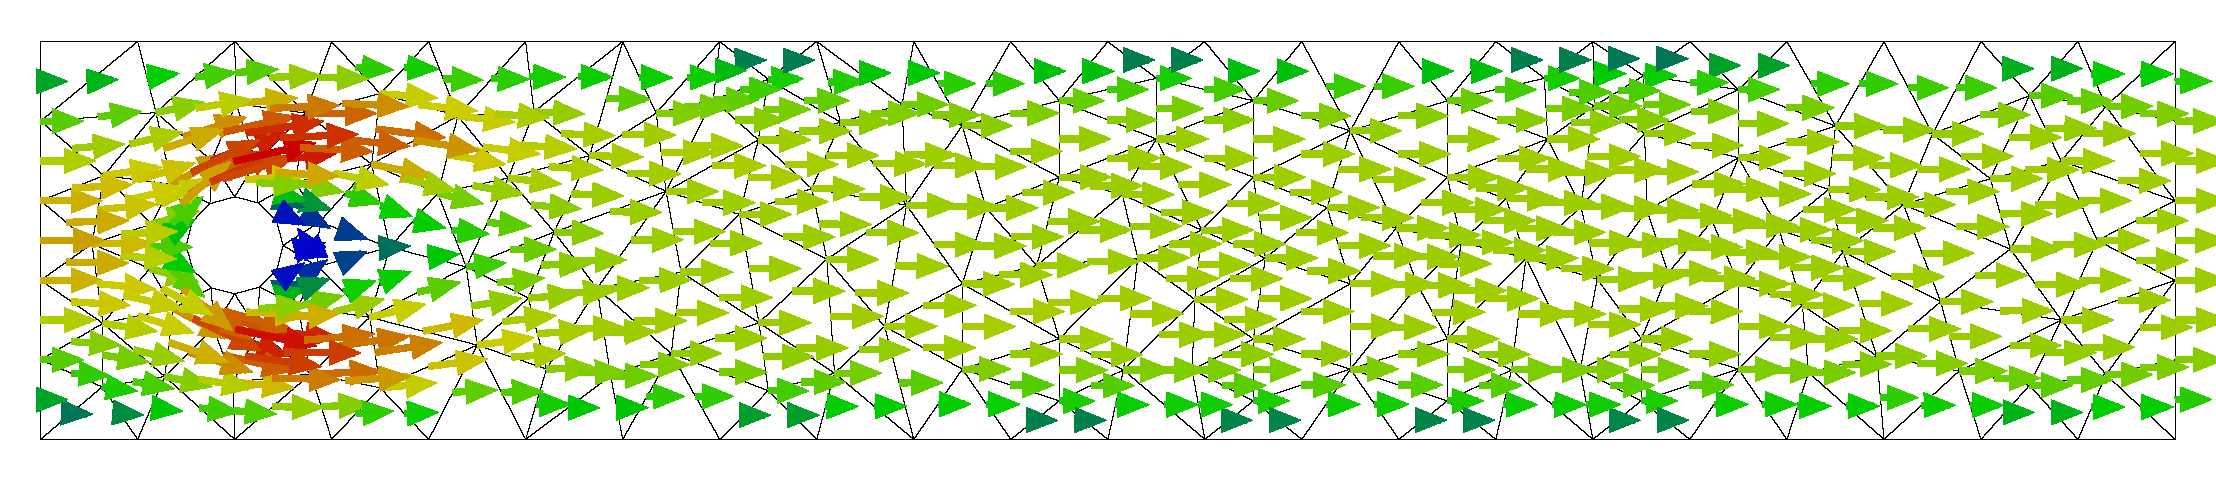
\includegraphics[width=\textwidth]{Figures/01_introduction/P2P1_adv_diff_100.pdf}
\caption{Solution for laminar flow via \crefrange{eq:adv-diff-split-advect}{eq:adv-diff-split-diffuse} after 100 iterations with $\Delta t = 0.01$.}\label{fig:advection-diffusion-plot}
\end{figure}

\section{Conclusion}
We have decided to further develop the three way splitting method. This is based on a few properties. First, the numerical experiment did not show any problems with the accuracy for the given task. Second, the semi-Lagrangian advection method is perfect for multithreaded CPU and GPU implementation. Third, the method can be used with an arbitrary step size and the step size is not tied to the spatial step (element size).